%===================================================
%================== DOCUMENT CLASS
%===================================================
\documentclass[runningheads,11pt,a4paper,english,llncs]{Misc/llncs}

%===================================================
%================== PACKAGES
%===================================================
%------------------------------------------------------------------------
% TeX and LaTeX macros
%------------------------------------------------------------------------
%
% In math formulas we use italic instead of mathitalic
%
\makeatletter
% ~ gives a \; space in math mode
\def~{\ifmmode\;\else\penalty\@M\ \fi}
%  Italic in mathematical formulas
\def\@setmcodes#1#2#3{{\count0=#1 \count1=#3
  \loop \global\mathcode\count0=\count1 \ifnum \count0<#2
  \advance\count0 by1 \advance\count1 by1 \repeat}}
\DeclareSymbolFont{italic}{OT1}{\rmdefault}{m}{it}
\let\mathit\undefined
\DeclareSymbolFontAlphabet{\mathit}{italic}
\edef\@tempa{\hexnumber@\symitalic}
\@setmcodes{`A}{`Z}{"7\@tempa41}
\@setmcodes{`a}{`z}{"7\@tempa61}
\makeatother
%
% \begin{asm} ... \end{asm}
%
\newdimen\asmindent     
\asmindent=\parindent
\newcount\asmi
\def\inc{\global\advance\asmi by 1}
\def\dec{\global\advance\asmi by-1}
\def\nl{{}$\par\hangindent\asmi em
  \noindent\kern\asmi em\ignorespaces$} 
\def\asmskip{{}$\par\smallskip\hangindent\asmi em
  \noindent\kern\asmi em\ignorespaces$}

%%%%%%%%%%%%%%%%%%%%%%%%%%%
\def\asm{\global\asmi=0 
 \def\+{\inc\nl}
 \def\-{\dec\nl}
 \def\\{\nl}
 %%% Added by Paolo 2018-06-25:
 \setlength{\parskip}{0pt}
 %%%
 \begin{trivlist}\item[]\leftskip=\asmindent\relax$}
%%%%%%%%%%%%%%%%%%%%%%%%%%%

\def\endasm{$\end{trivlist}}
%\mathindent=\asmindent
%
% \begin{asmarray}
%    f(s_1) & := t_1 \\
%    f(s_2) & := t_2 
% \end{asmarray}
%
\def\asmarray{\begin{array}[t]{@{}l@{\;}l@{\;}l@{}}}
\def\endasmarray{\end{array}}
%
%
%
\def\asmcomment#1{\quad\hbox{// #1}}
%
%  \begin{subasm} ... \end{subasm}
%
\newcount\asmii
\def\subasm{\vtop\bgroup\asmii=0\normalbaselines
 \def\nl##1{$\egroup\advance\asmii by##1\relax\hbox\bgroup\hskip\asmii em$}
 \def\\{\nl{0}}
 \def\+{\nl{1}}
 \def\-{\nl{-1}}
 \hbox\bgroup\hskip\asmii em$}
\def\endsubasm{$\egroup\egroup}
%
% Keywords in ASM code
%
\def\ASM#1{\hbox{\sc#1}}        % rule names and macros
\def\ASMIND#1{\ASM{#1}\index{#1@{\sc#1}}}
\def\AWAIT   {\mathrel{\mathbf{await}}}
\def\AND     {\mathrel{\mathbf{and}}}
\def\CASE    {\mathrel{\mathbf{case}}}
\def\CHOOSE  {\mathrel{\mathbf{choose}}}
\def\CREATE  {\mathrel{\mathbf{create}}}
\def\NEW  {\mathrel{\mathbf{new}}}
\def\DO      {\mathrel{\mathbf{do}}}
\def\ELSE    {\mathrel{\mathbf{else}}}
\def\ELSEIF  {\mathrel{\mathbf{elseif}}}
\def\FORALL  {\mathrel{\mathbf{forall}}}
\def\FORSOME  {\mathrel{\mathbf{forsome}}}
\def\FOREACH  {\mathrel{\mathbf{foreach}}}
\def\THEREISNO  {\mathrel{\mathbf{thereisno}}}
\def\FROM  {\mathrel{\mathbf{from\colon}}}
\def\FOR  {\mathrel{\mathbf{for\colon}}}
\def\TO  {\mathrel{\mathbf{to\colon}}}
\def\IF      {\mathrel{\mathbf{if}}}
\def\IFF      {\mathrel{\mathbf{iff}}}
\def\IMPORT  {\mathrel{\mathbf{import}}}
\def\IN      {\mathrel{\mathbf{in}}}
\def\LET     {\mathrel{\mathbf{let}}}
\def\SELF    {\mathrel{\mathbf{self}}}
\def\MATCH    {\mathrel{\textbf{match}}}
\def\NOT     {\mathrel{\mathbf{not}}}
\def\OF      {\mathrel{\mathbf{of}}}
\def\OR      {\mathrel{\mathbf{or}}}
\def\PAR     {\mathrel{\mathbf{par}}}
\def\SEQ     {\mathrel{\mathbf{seq}}}
\def\SKIP    {\mathrel{\mathbf{skip}}}
\def\THEN    {\mathrel{\mathbf{then}}}
\def\WHERE   {\mathrel{\mathbf{where}}}
\def\WHILE   {\mathrel{\mathbf{while}}}
\def\UNDEF   {\mathrel{\mathbf{undef}}}
\def\UNTIL   {\mathrel{\mathbf{until}}}
\def\WHEN   {\mathrel{\mathbf{when}}}
\def\WITH    {\mathrel{\mathbf{with}}}
\def\STEP    {\mathrel{\mathbf{step}}}
\def\STEPWISE    {\mathrel{\mathbf{stepwise}}}
\def\SEQ    {\mathrel{\mathbf{seq}}}
\def\RESULT  {\mathrel{\mathbf{result}}}
\def\CALL  {\mathrel{\mathbf{Call}}}
\def\LOCAL    {\mathrel{\mathbf{local}}}
\def\ADDGUARD {\mathrel{\mathbf{addGuard}}}
\def\ADDUPD   {\mathrel{\mathbf{addUpd}}}
\def\ADDRULE  {\mathrel{\mathbf{addRule}}}
\def\MINUSRULE  {\mathrel{\mathbf{minusRule}}}
%\def\TO      {\mathrel{\mathbf{to}}}
%
% Including figures
%
\def\includefig#1#2{\centering\medskip
  \includegraphics[scale=#1]{fig/#2}
  \medskip}
%
% References to paragraphs in the ECMA standard for C#
%
\def\ecma#1{\cite[\S#1]{ecma334}}
%
%  Environments for definitions and theorems
%
%\theorembodyfont{\rm}
%\newtheorem{definition}[subsection]{Definition}
%\newtheorem{lemma}[subsection]{Lemma}
%\newtheorem{theorem}[subsection]{Theorem}
%\newtheorem{proposition}[subsection]{Proposition}
%\newtheorem{corollary}[subsection]{Corollary}
%\newtheorem{example}[subsection]{Example}
%\newtheorem{remark}[subsection]{Remark}
%\newtheorem{constraint}[subsection]{Constraint}
\def\proof{\trivlist\item[]{\bf Proof.}}
\def\endproof{$\Box$\endtrivlist}
%
% enumerate and itemize (smaller skips) from "latex.ltx"
%
\makeatletter
\def\enumerate{%
  \ifnum \@enumdepth >\thr@@\@toodeep\else
    \advance\@enumdepth\@ne
    \edef\@enumctr{enum\romannumeral\the\@enumdepth}%
      \expandafter
      \list
        \csname label\@enumctr\endcsname
        {\usecounter\@enumctr\def\makelabel##1{\hss\llap{##1}}
         \itemsep 0pt\parskip 0pt\parsep 0pt\topsep\smallskipamount}%
  \fi}
\def\itemize{%
  \ifnum \@itemdepth >\thr@@\@toodeep\else
    \advance\@itemdepth\@ne
    \edef\@itemitem{labelitem\romannumeral\the\@itemdepth}%
    \expandafter
    \list
      \csname\@itemitem\endcsname
      {\def\makelabel##1{\hss\llap{##1}}
       \itemsep 0pt\parskip 0pt\parsep 0pt\topsep\smallskipamount}%
  \fi}
\makeatother
%
% items in itemize
%
\def\bull{\vrule height .9ex width .8ex depth -.1ex}
\def\labelitemi{\bull}
%
%
%
\def\cs#1{C\#$_{\mathcal{#1}}$}
\def\lang#1{L$_{\mathcal{#1}}$}
%
% Positions
%
\def\pos#1{{}^{#1}}
\def\termPos{\blacktriangleright}
\def\cursor{\pos{\termPos}}
%
%
%
\def\sup{\hbox{sup}}
\def\c#1{\texttt{#1}}           % code
\def\N#1{\textit{#1}}           % non terminal symbols
\def\T#1{\hbox{`\texttt{#1}'}}  % terminal symbols
\def\A#1{\hbox{\sc#1}}          % ASM rules
\def\D#1{#1}                    % dynamic functions
\def\U#1{#1}                    % universes
\def\C#1{#1}                    % constructors
\def\rdef{\equiv}
\def\lbr{\c{\char`\{}}
\def\rbr{\c{\char`\}}}
\def\mb{\hbox{::}}
\def\map#1#2{\textbf{Map from}~#1~\textbf{to}~#2}
\def\cat{\cdot}
\def\adots{\mathinner{\ldotp\ldotp}}
%
%
% macros.tex ends here

%\include{Misc/json}
%\include{Misc/bsl}
\usepackage{etex}
\reserveinserts{28}
\newcommand{\todo}[1]{
 \noindent{\newline \color{red}
 \framebox[\textwidth][t]{%
  \parbox[t]{0.9\textwidth}{\textcolor{red}{TODO: #1}}                                                                                     
}}}
\usepackage{listings}
\lstset{
  basicstyle=\ttfamily,
  columns=fullflexible,
  breaklines=true,
  postbreak=\mbox{\textcolor{red}{$\hookrightarrow$}\space},
}
\usepackage{graphicx}
\usepackage{acronym}
\usepackage{ifthen}
\usepackage{substr}
\usepackage{color}
\usepackage{fixltx2e}
\usepackage[left=2cm, top=2cm, right=2cm, bottom=2cm]{geometry}
%\usepackage{subfigure}
\usepackage{array}  
\usepackage[figuresright]{rotating}          
\usepackage{url}
\usepackage{tikz}
\usetikzlibrary{trees}
%\usepackage{enumerate}
\usepackage[shortlabels]{enumitem}
\usepackage{epsfig}
\usepackage{colordvi}
\usepackage{makeidx}
\usepackage{index}
\usepackage[absolute]{textpos}
\setlength{\TPHorizModule}{\paperwidth}
\setlength{\TPVertModule}{\TPHorizModule}
\textblockorigin{-6mm}{0mm}
\usepackage[%
      breaklinks=true,%
      colorlinks=true,%           no frame around URL
      urlcolor=LINK_COLOR,%            no colors
      menucolor=LINK_COLOR,%           no colors
      linkcolor=LINK_COLOR,%           no colors
      pagecolor=LINK_COLOR,%           no colors
      bookmarks=true,%            tree-like TOC
      bookmarksopen=false,%       expanded when starting
      hyperfootnotes=true,%       no referencing of footnotes, does not compile
      citecolor=CITE_COLOR,%           black cites
      filecolor=black,%           black files%
      hyperindex=true,%
      hyperfigures=true%
]{hyperref}
\usepackage{bookmark}
\usepackage{booktabs}
\usepackage{dsfont}
\usepackage{wallpaper}
\usepackage{mathtools,cancel}
\usepackage{soul}
\usepackage{float}
\usepackage{setspace}
%\usepackage{morefloats}
%\usepackage{mdwlist}
\usepackage{amsmath,amssymb,amscd,diagrams,bm,amsfonts}
\let\proof\relax
\let\endproof\relax
\usepackage{amsthm}
\usepackage{tabularx, graphics, longtable, multirow, makecell}

%%%%%%% Added by Paolo 2018-03:
\usepackage[justification=centering]{caption}
\usepackage{eurosym}
%%%%%%%%%%%%%%%%%%%%%%

%\usepackage[title]{appendix}


%TIKZ
\usepackage{tikz}
\usepackage{tikz-cd}
\usetikzlibrary{trees,snakes}
\usetikzlibrary{arrows,automata}
\usetikzlibrary{matrix,arrows,positioning}
\usetikzlibrary{mindmap,backgrounds}
\usetikzlibrary{shapes}
\usepackage{verbatim} %for comment out some texts

%%%%%%%%%%%%%%%%%%%%%%%%%%%%%%%
%%%%%%%%%%%%%%%%%%%%% Egon's commands:
\usepackage{latexsym}
\ifx\pdfoutput\undefined
  \message{We are running LaTeX.} 
%PD  \usepackage[dvips]{graphicx}
%PD  \DeclareGraphicsExtensions{.eps}
%PD  \usepackage[hypertex,bookmarks=false]{hyperref}
\else
  \message{We are running PDFLaTeX.}
%PD  \usepackage[pdftex]{color}
%PD  \usepackage[pdftex]{graphicx}
%PD\DeclareGraphicsExtensions{.jpg,.pdf}
%PD  \DeclareGraphicsExtensions{.pdf}
%PD  \usepackage[pdftex,bookmarks=false]{hyperref}
%PD  \hypersetup{colorlinks={true},
%PD            linkcolor={blue},
%PD            citecolor={blue},
%PD            urlcolor={blue},
%PD            plainpages={false}
%PD  }
\fi
%%%%%%%%%%%%%%%%%%%%%%%%%%%%%%%
%%%%%%%%%%%%%%%%%%%%%%%%%%%%%%%

%===================================================
%================== THEOREMS
%===================================================
\theoremstyle{plain}
\newtheorem{thm}{Theorem}
\newtheorem{cor}[thm]{Corollary}
\newtheorem{lem}[thm]{Lemma}
\newtheorem{prop}[thm]{Proposition}
\newtheorem{defin}[thm]{Definition}
\newtheorem{rmrk}[thm]{Remark}

\allowdisplaybreaks


%===================================================
%================== COLOURS
%==================================================

\definecolor{green}{rgb}{0,0.6,0} 
\definecolor{gray}{rgb}{0.6,0.6,0.6} 
\definecolor{red}{rgb}{1,0,0} 
\definecolor{blue}{rgb}{0,0,1} 
\definecolor{purple}{rgb}{0.5,0,0.5} 
\definecolor{yellow}{rgb}{0.25,0.25,0} 
\definecolor{turquoise}{rgb}{0,0.5,0.5}
\definecolor{brown}{rgb}{0.6,0.2,0.1}

\definecolor{LINK_COLOR}{rgb}{0,0,0.7}
\definecolor{CITE_COLOR}{rgb}{0,0.5,0}
\definecolor{lightblue}{rgb}{0,0,1}
\definecolor{light-gray}{gray}{0.95}
\def\red#1{\textcolor[rgb]{1.0,0.0,0.0}{#1}}
\def\green#1{\textcolor[rgb]{0.0,0.8,0.1}{#1}}
\def\blue#1{\textcolor[rgb]{0.0,0.0,1.0}{#1}}

%===================================================
%================== LAYOUT
%===================================================
\parindent=0cm
%\setlength{\parskip}{1.0\baselineskip plus 0.5ex minus 0.2ex}
\abovecaptionskip=0cm
\hyphenpenalty=5000
\tolerance=1000 
\floatsep=1in
\allowdisplaybreaks
\def \constzeroindent {0cm}
\def \constfirstindent {0.5cm}
\def \constsecondindent {1cm}
\newenvironment{mycustomindent}[1]
{\setlength{\parindent}{#1}}
{\setlength{\parindent}{\constzeroindent}}
\newcommand{
	\firstindent}[1]{
	\begin{mycustomindent}{\constfirstindent}
	\begin{tabular}{@{}p{12cm}@{}}
	#1 \\
	\end{tabular}
	\end{mycustomindent}
}
\newcommand{
	\secondindent}[1]{
	\begin{mycustomindent}{\constsecondindent}
	\begin{tabular}{@{}p{12cm}@{}}
	#1 \\
	\end{tabular}
	\end{mycustomindent}
}
\newenvironment{packed_item1}{
\begin{itemize}[topsep=0pt, partopsep=0pt]
  \setlength{\itemsep}{5pt}
  \setlength{\parskip}{0pt}
  \setlength{\parsep}{0pt}
}{\end{itemize}}
\newenvironment{packed_item2}{
\begin{itemize}[topsep=0pt, partopsep=0pt]
  \setlength{\itemsep}{0pt}
  \setlength{\parskip}{0pt}
  \setlength{\parsep}{0pt}
}{\end{itemize}}
\newenvironment{packed_enumerate}{
\begin{enumerate}[topsep=0pt, partopsep=0pt]
  \setlength{\itemsep}{5pt}
  \setlength{\parskip}{0pt}
  \setlength{\parsep}{0pt}
}{\end{enumerate}}
% The following commands are to get rid of the extra space around section and subsection titles:
% Save the class definition of \subparagraph:
\let\llncssubparagraph\subparagraph
% Provide a definition to \subparagraph to keep titlesec happy:
\let\subparagraph\paragraph
\usepackage[compact]{titlesec}
\usepackage{dblfloatfix,caption,subcaption}
\titlespacing{\section}{0pt}{12pt}{*0}
\titlespacing{\subsection}{0pt}{6pt}{0pt}
\titlespacing{\subsubsection}{0pt}{6pt}{0pt}
% Force section numbering to follow chapter numbering:
\usepackage{chngcntr}
\counterwithin{section}{chapter}
\counterwithin{figure}{chapter}
%\counterwithin{theorem}{chapter}
%\counterwithin{lemma}{chapter}
%\counterwithin{definition}{chapter}
%%%%%%%%%%%%%%%%%%%%%%%%%%%%
% Allow line breaks in long list of citations that would extend into the margin:
\usepackage{breakcites}
%%%%%%%%%%%%%%%%%%%%%%%%%%%%%%%%%%%%%%

\usepackage{pdfpages}
\pagestyle{headings}

\renewcommand{\rightmark}{INTERLACE Project (Grant no.~754494)}
\renewcommand{\leftmark}{D4.2}
\setcounter{tocdepth}{2}

\usepackage{tocloft}
\setlength\cftparskip{0pt}
\setlength\cftbeforechapskip{12pt}

%\renewcommand{\cfttoctitlefont}{\normalfont\MakeUppercase}

\usepackage{abstract}
\renewcommand{\abstractnamefont}{\large \bfseries}
%\setlength{\abstitleskip}{-\absparindent}
\renewcommand{\abstractname}{Abstract}

\setlength{\parskip}{12pt}

\begin{document}
%===================================================
%================== TITLE
%===================================================

\thispagestyle{empty}

\includepdf[pages=-, scale=1.0]{Misc/Front}

%===================================================
%================== ABSTRACT
%===================================================
\thispagestyle{empty}

\begin{abstract}
\normalsize

This deliverable is much briefer than it could have been. The project ran out of time and funds before we reached the final
workpackage on testing. In this short report we provide a short outline of the commercialisation plan.


\end{abstract}

\newpage

%===================================================
%================== TABLE OF CONTENTS
%===================================================
\tableofcontents


%===================================================
%================== CHAPTERS
%===================================================
\chapter{Introduction}
\label{ch:Introduction}

\vspace{-1cm}
\begin{center}
Giuseppe Littera and Paolo Dini
\end{center}

The component testing of the platform was performed only at an essential level, as reported in deliverable D3.2 \cite{INTERLACE_D32}, due to lack of time and funding. Not having had the time to perform the component acceptance testing, we could not perform the field tests either. We expect the component testing to be completed sometime in 2019 and the field testing probably in 2020. All updates will be shared on GitHub\footnote{\url{https://github.com/InterlaceProject/InterlaceBlockchain}} and/or on the project's website.\footnote{\url{https://www.interlaceproject.eu/}} Here we add a few words on the commercialisation plan, which has evolved significantly over the past few years.

The overarching objective of the project was to develop, collaboratively, an open source and blockchain-based transactional platform for mutual credit. This was motivated by a desire to build in-house blockchain expertise in order to remain competitive, but also in order to achieve better scalability as the Sardex platform is extended to additional circuits in Italy and beyond. Although INTERLACE has laid the groundwork for such a system, as shown in deliverable D2.3 \cite{INTERLACE_D23} the system involves many other components beyond the transactional platform. Therefore, its overhaul and redesign is going to take a significantly greater amount of resources than this project could provide. It follows that the future business model and commercialisation plan need to be convincing for the size of venture capital (VC) investment needed. The next chapter provides a brief outline of a possible plan.

\newpage

\chapter{Commercialisation Plan}
\label{ch:commercialisation}

\vspace{-1cm}
\begin{center}
Giuseppe Littera, Giovanni Dini and Paolo Dini
\end{center}

For Sardex ``commercialisation'' is only part of the story -- and of the requirement. Since the circuit is based on high levels of trust and on the real economy, in fact, the social dimension is not just a nice ``add-on'' but, rather, it is the part of the circuit that must be protected most carefully since this is where the value and success of Sardex are created and originated. On the other hand, Sardex is a B2B mutual credit circuit in support of trade and, therefore, the economic dimension is equally important.

Since the commercialisation plan we outline here reflects a balance between these two requirements, it should be regarded as the beginnings of a governance framework, company structuring model, and business model all at the same time. In other words, the future of the Sardex financial service and of the technology platform that enables it, as it scales beyond Italy and Europe, concerns the governance and sustainability aspects of the community of users and developers as much as the economic viability of the ``mothership'', Sardex S.p.A. This multi-dimensional sustainability requirement has led us towards a non-trivial possible structuring of the company which, furthermore, is able to evolve over time and in response to the growth of the initiative in number of circuits and geographical reach.

A good example that can be used as a ``reference model'' and starting point to describe this approach is provided by the Robert Bosch Gmbh company.\footnote{\url{https://en.wikipedia.org/wiki/Robert_Bosch_GmbH}} The motivation of the Bosch family was similar to ours in the sense that they had objectives that were not solely commercial. Therefore, it was important to make it difficult or impossible for their company to be made public (listed on the stock exchange) and become hostage to the shareholders. At the same time, they wanted to retain competitiveness to protect the jobs of their employees. As shown in Figure \ref{fig:bosch}, these apparently conflicting requirements were met by an unusual company structure whose main characteristic is the separation between the holders of the equity (and therefore the recipients of the dividends) and the holders of the voting rights (and therefore the people who make long-term decisions about the company).

\begin{figure}[h]
\centering
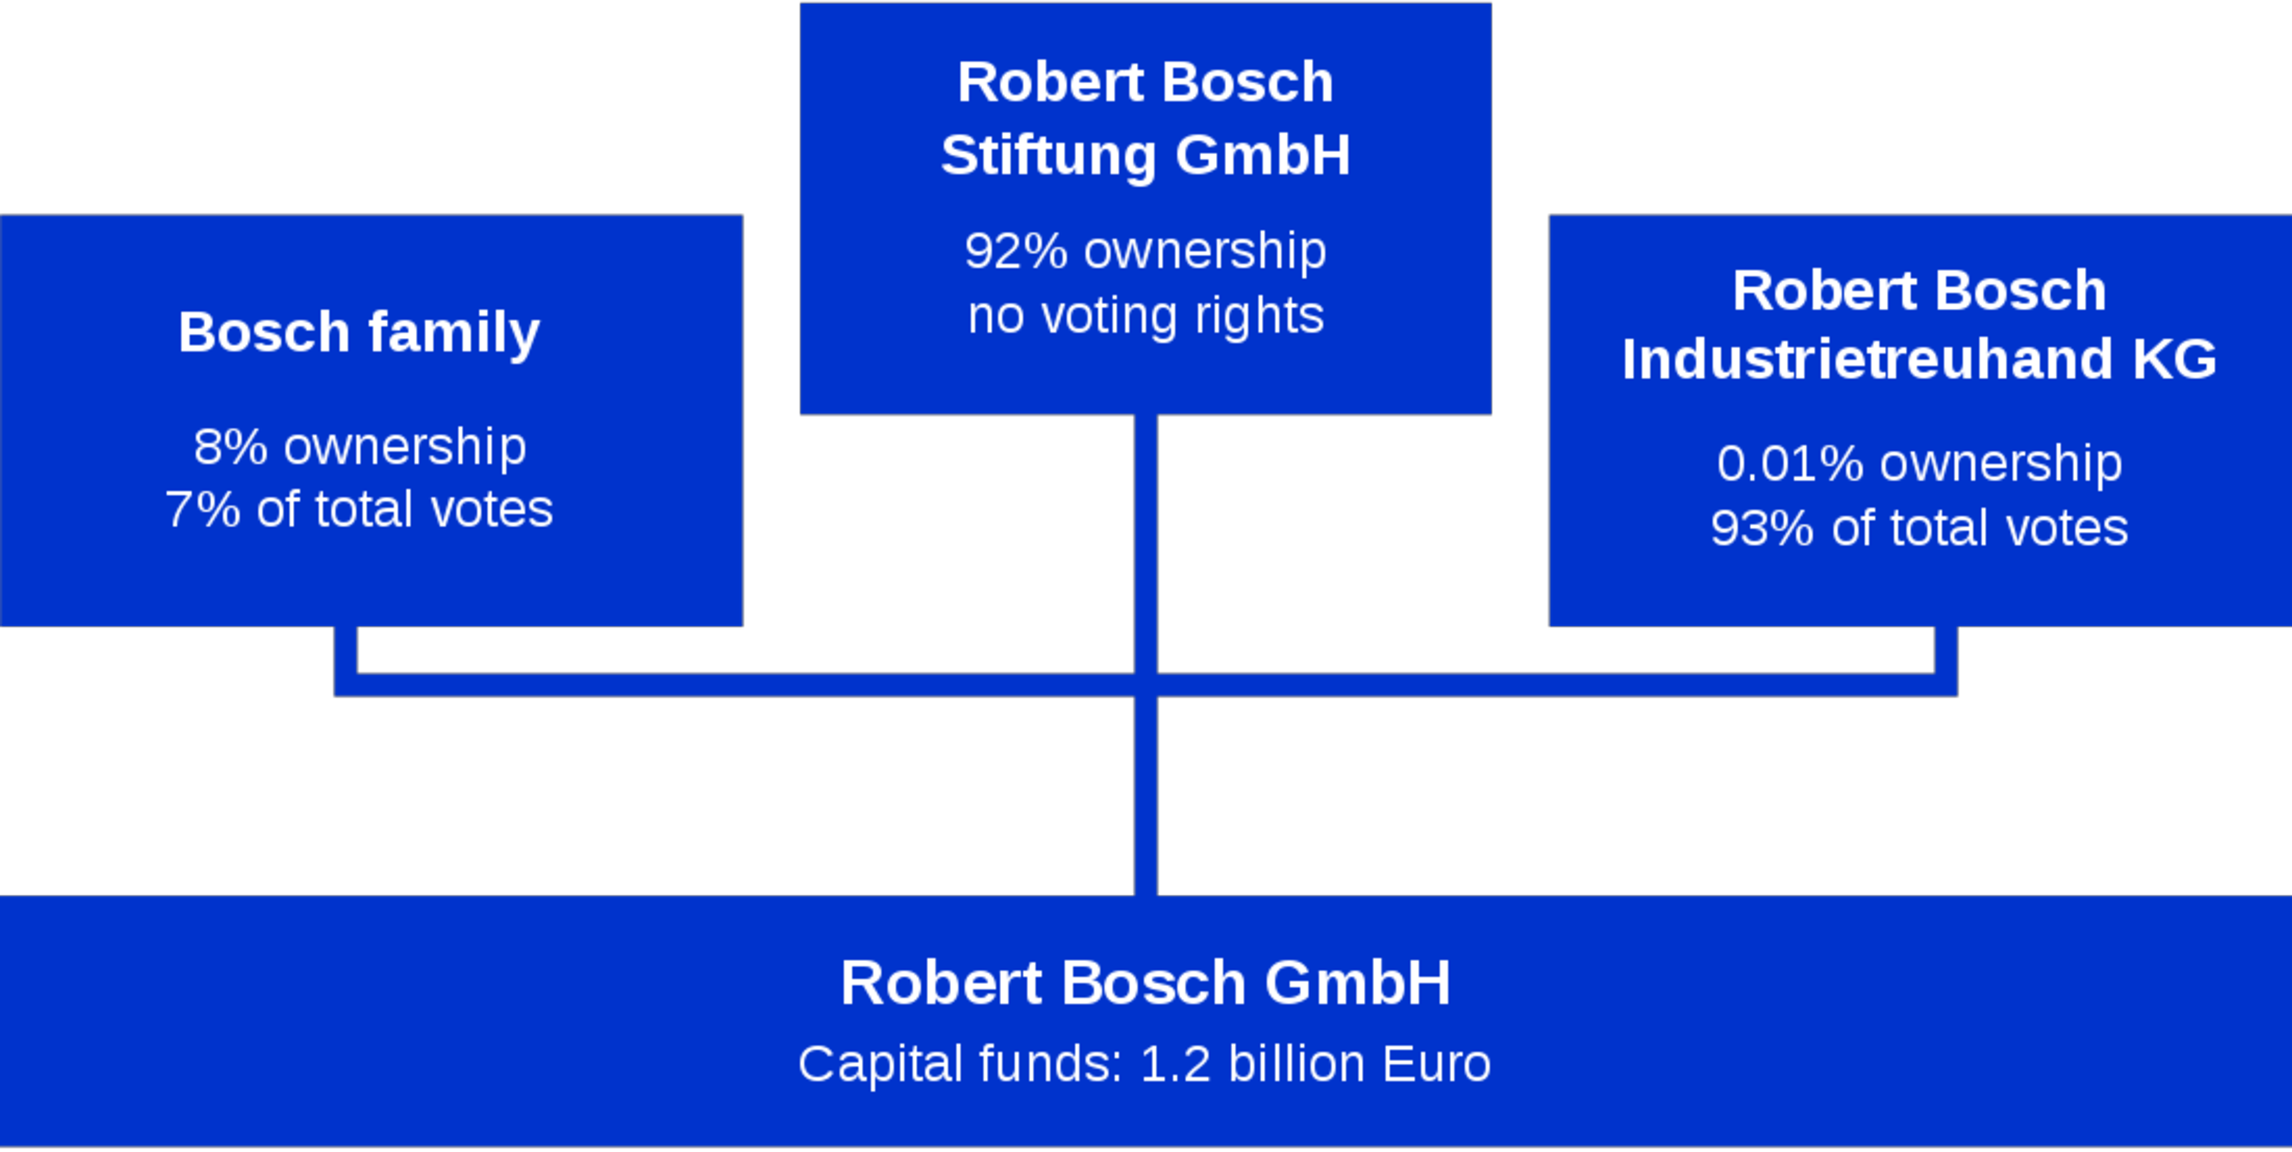
\includegraphics[width=12 cm]{Figures/Bosch}
\caption{\bf \small Robert Bosch Gmbh company structure}
\label{fig:bosch}
\end{figure}

Most of the equity (92\%) is held by the non-profit Bosch Foundation (Stiftung) which, however, has no control. The control (93\% of the votes) is held by the Bosh Industrial Trust (Industrietreuhand), which is populated by experienced business persons who are elected to this post and by past Managing Directors; however, they have only 0.01\% of the equity. The Bosch family retains a small amount of equity and control. Finally, the company itself is run by people who are hired and appointed for this job. As explained by the wikipedia article, about 5\% of the dividends are distributed to the Bosch charitable foundation, while the bulk of what's left is reinvested in the company. This enables it to sustain an R\&D budget of approximately 9\% of the revenue, which is twice the industry average and enables Bosch to remain competitive.

The Sardex mutual credit system, in practical terms, provides working capital at 0\% interest to small and medium-sized enterprises (SMEs). This is important because SMEs are always vexed by cashflow problems; asking for a credit line from banks is seldom successful; and, when they succeed, such short-term loans are very expensive. The root of this problem can be found in the Basel accords on banking regulation, whose purpose was to protect the savings of e.g.\ pension funds from the financial speculative practices of commercial banks. This reasonable objective has had as an unintended deleterious consequence the tightening of credit towards any commercial enterprise regardless of whether it engages or not in speculative practices. Furthermore, the risk weightings allocated to credit applicants are disproportionally unfavourable towards SMEs. In other words, in an effort to keep the financial economy in check the real economy has also been strongly curtailed. But, crucially, whereas most large companies have their own financial arms and a large enough cashflow to be able to work around these restrictions and continue operating, most SMEs are chronically vexed by cashflow problems, especially in weak economies such as, in Europe, those on the Mediterranean basin.

What Sardex offers the SMEs that join its circuit(s), therefore, is extremely valuable and a useful intervention that creates greater stability in the SME sector. In order to function, however, mutual credit requires mutual trust. Since trust is based on social relations, it follows that a mutual credit system works best at small geographical scales. Hence, the only possible way it can scale to international level while retaining its core principle of locally-rooted social relations and trust is as a set of loosely linked circuits that share some infrastructural aspects and retain some level of local autonomy.

One possible approach that seems able to capture these requirements is to aim for different levels of integration at different levels of the stack. Thus, the blockchain-based transactional platform and the suite of microservices surrounding it are likely to be held and controlled by a single company that could scale and even become public, thereby attracting more traditional VC investors. Such a company would be linked to a non-profit company that contains all the circuits and whose ultimate ownership is likely to be in part by the SMEs themselves. A legal personality for the non-profit company that has attracted our attention is the Stewardship model \cite{Karns2011}, which explicitly puts a social purpose at the centre of its mission and vision. Figure \ref{fig:structure} summarises these points graphically.

\begin{figure}[h]
\centering
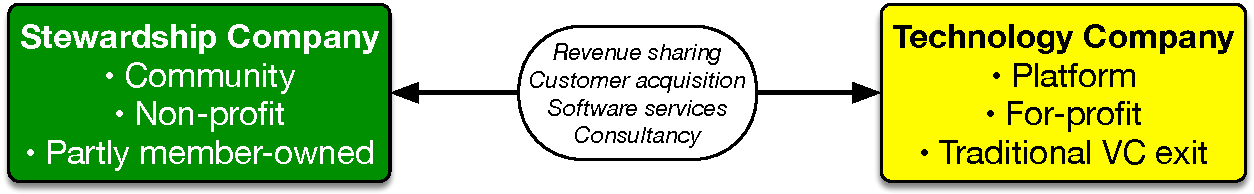
\includegraphics[width=16 cm]{Figures/structure}
\caption{\bf \small Possible future company structure for sustainability and scalability}
\label{fig:structure}
\end{figure}

In summary, the lesson from the first 10 years of the Sardex company's life is that the business model and the technology are always evolving, as new needs and product ideas emerge. As we have seen over the past 2.5 years since the project idea was formulated, this trend is even stronger with blockchain technologies. Therefore, the INTERLACE platform is also likely to continue to evolve, building on the basis that this project has enabled and drawing together and ever-growing community of developers, SMEs, and investors to continue to offer an invaluable service to SMEs in a new and more constructive interpretation of `Finance' in the service of the real local economy.






















\chapter*{References}
\renewcommand{\section}[2]{}
\setlength{\parskip}{0.8\baselineskip}
\bibliographystyle{plainurl}
{\small
\addcontentsline{toc}{chapter}{References}
\bibliography{Bib/BioComp_References}}



%===================================================
%================== APPENDIX
%===================================================
%\begin{appendix}
%\section*{Appendix}
%\includepdf[pages={-}]{sections/4-CaSM/CaCycleAsm.pdf}
%\end{appendix}

\end{document}
